%%% Analyse af optimering af udgangsfilter %%%

\section{Udgangsfilter}
I 2. itertion blev udgangsfilteret realiseret ved fire $56\micro F$ film kondensatorer i parallel. Filteret er vist på figur~\ref{fig:udgangsfilter_2} hvor selve filteret er de fire blå kondensatorer, og udgangen er bananstikkene placeret til venstre. 


\begin{figure}[H]
	\center
	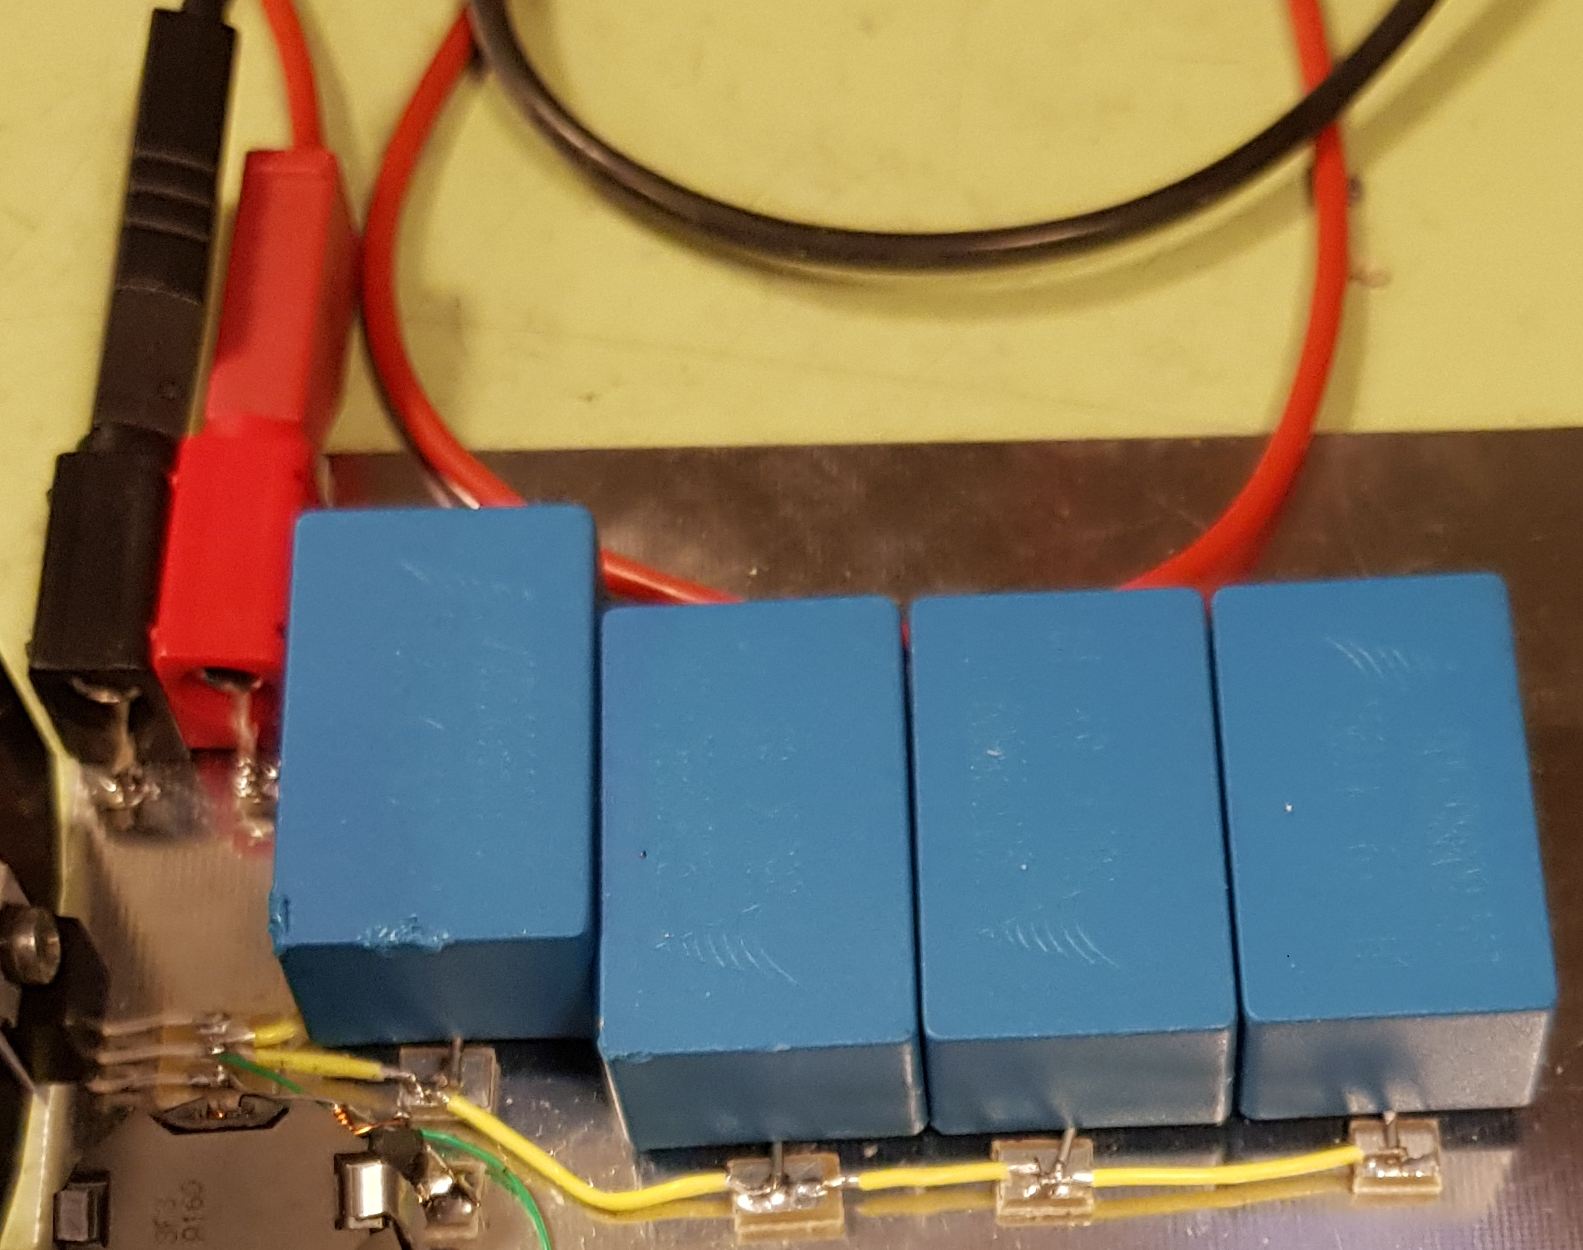
\includegraphics[max width=0.7\linewidth]{/tex/3iteration/billeder/Analyse/Udgangsfilter_2iteration.png}
	\caption{Implementeret udgangsfilter - 2. iteration}
	\label{fig:udgangsfilter_2}
\end{figure}

Denne implementering af udgangsfilteret, medførte switchin-spikes på udgangen op mod $5V pk-pk$. Dette er vist på figur~\ref{fig:output_2}, hvor kanal 1 viser udgangen, og kanal 2 viser MOSFET'ens gate. Disse spikes ønskes mindsket. I afsnit~\ref{output_cap} blev det beskrevet, at det som hovedregel kan antages, at en ledning har en selvinduktion på $1nH/mm$. Bruges den antagelse på udgangsfilteret, kan ledningerne mellem kondensaterne moduleres som spoler. Det betyder, at hver kondensator er en del af et LC-filter, som hver især filtrere højfrekvente signaler på udgangen. 


\begin{figure}[H]
	\center
	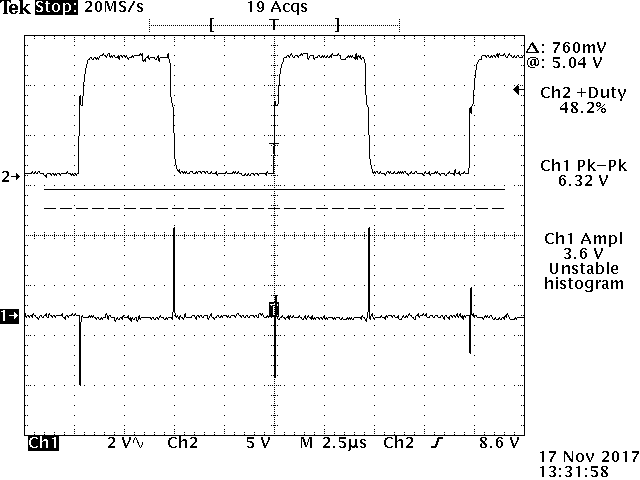
\includegraphics[max width=0.7\linewidth]{/tex/2iteration/billeder/Realisering/Output_26V.png}
	\caption{Output - 2. iteration}
	\label{fig:output_2}
\end{figure}

Det antages at hver ledning i gennemsnit er ca. $30mm$, hvilket giver en selvinduktion på ca. $30nH$. Der regnes en knækfrekvens for filteret ved ligning~\ref{out_filter}. Det viser, at knækfrekvensen for filtret ligger tæt på den brugte switch-frekvens, hvilket ikke er optimalt. Det vurderes dog, at den ligger højt nok, til ikke at have en påvirkning på det egentlige udgangssignal. Tilsammen vil de fire kondensatorer dermed virke som et 8. ordensfilter med en knækfrekvens på ca. $122.8k\hertz$. Ud fra den analyse vælges det, at flytte udgangen til den anden ende af udgangsfilteret, for dermed at udnytte denne filtrering. 

\begin{equation} \label{out_filter}
f = \frac{1}{2 \cdot \pi \cdot \sqrt{C_{out} \cdot L_{out}}} = \frac{1}{2 \cdot \pi \cdot \sqrt{56\micro F \cdot 30nH}} = 122.8k\hertz
\end{equation}

I kombination med kondensatorens resonans frekvens på $108k\hertz$, regnet i afsnit~\ref{output_cap}, burde der findes en ny kondensator i en senere iteration. 

